
\documentclass[12pt]{article}
\usepackage[notext]{stix}
\usepackage{step}
\usepackage[T1]{fontenc}
\usepackage{amsmath}
\usepackage{amsfonts}
\usepackage[margin=2.5cm]{geometry}
\usepackage{titling}
\usepackage{listings}
\usepackage{titlesec}
\usepackage{parskip}
\usepackage[dvipsnames]{xcolor}
\usepackage{tikz}
\usepackage{hyperref}
\usepackage{graphicx}
\graphicspath{{LaTex\space Images/}}
\DeclareGraphicsExtensions{.pdf,.jpeg,.png}

\hypersetup{
    colorlinks=true,
    linkcolor=blue,
    filecolor=blue,      
    urlcolor=cyan,
    pdftitle={Overleaf Example},
    pdfpagemode=FullScreen,
    }

\usetikzlibrary{chains, scopes}
\tikzset{memory box/.style={
        draw, fill=#1, minimum width={width("Memory UVWXYZ")+6pt},
        align=center, minimum height=4ex,
        outer sep=0pt, % this will make the borders overlap nicely
    },
    memory size/.style={
        anchor=south east, font=\tiny, inner sep=1pt
    },
    memory address/.style={
         font=\tiny\ttfamily, inner ysep=1pt, inner xsep=3pt,
         anchor=#1 east,
    },
}

\lstset{ 
    language=C++, % choose the language of the code
    basicstyle=\fontfamily{pcr}\selectfont\footnotesize\color{red},
    keywordstyle=\color{red}\bfseries, % style for keywords
    numbers=none, % where to put the line-numbers
    numberstyle=\tiny, % the size of the fonts that are used for the line-numbers     
    backgroundcolor=\color{white},
    showspaces=false, % show spaces adding particular underscores
    showstringspaces=false, % underline spaces within strings
    showtabs=false, % show tabs within strings adding particular underscores
    frame=single, % adds a frame around the code
    tabsize=2, % sets default tabsize to 2 spaces
    rulesepcolor=\color{gray},
    rulecolor=\color{black},
    captionpos=b, % sets the caption-position to bottom
    breaklines=true, % sets automatic line breaking
    breakatwhitespace=false,
    commentstyle=\color{teal}, 
    emph={uint64_t},
    emphstyle=\color{blue}, 
}


\renewcommand\maketitlehooka{\null\mbox{}\vfill}
\renewcommand\maketitlehookd{\vfill\null}

\title{Operating Systems Notes}

\author{SubmergedDuck}
\date{\today}

\begin{document}
\begin{titlingpage}
\maketitle 
\end{titlingpage}

\newpage

\section{Page Tables: OSTEP {\hrule}}
\vspace{-1.5em}

    {\bf Paging.} {When memory is split into fixed-sized pieces. Inside one page,
    the offset tells "which byte within this page."} \par

    {\bf Page.} {A fixed size unit in a process's address space.} \par

\vspace{1em}
    {\bf Fig 1. 64-Byte Address Space in 128-Byte Physical Memory. TBC.}
\vspace{1em}
\begin{center}
    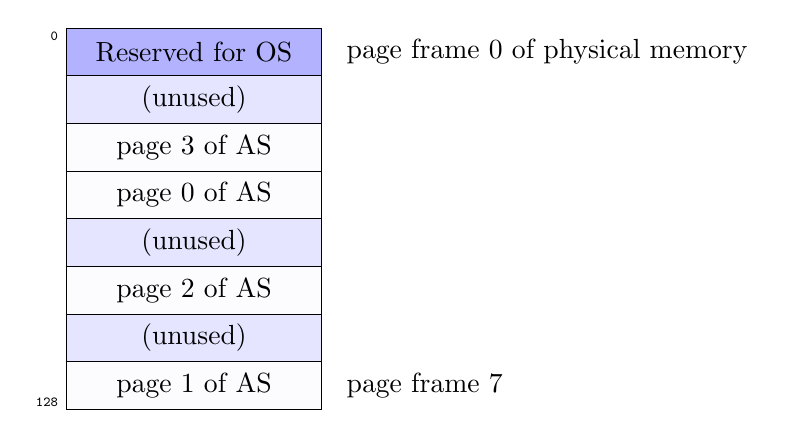
\begin{tikzpicture}[]
        \node [memory box=blue!1, anchor=south, label={[xshift=2mm]east:{page frame 7}}] (M0) {page 1 of AS};
        \node [memory box=blue!10, anchor=south] at (M0.north) (M1) {(unused)};
        \node [memory box=blue!1, anchor=south] at (M1.north) (M2) {page 2 of AS};
        \node [memory box=blue!10, anchor=south] at (M2.north) (M3) {(unused)};
        \node [memory box=blue!1, anchor=south] at (M3.north) (M4) {page 0 of AS};
        \node [memory box=blue!1, anchor=south] at (M4.north) (M5) {page 3 of AS};
        \node [memory box=blue!10, anchor=south] at (M5.north) (M6) {(unused)};        
        \node [memory box=blue!30, anchor=south, label={[xshift=2mm]east:{page frame 0 of physical memory}}] at (M6.north) (M7) {Reserved for OS};        

    %% Add the texts (just a couple, as example)
    %% add the size
        \node [memory size] at (M0.south east) {};
        \node [memory size] at (M1.south east) {};
    %% add the addresses. Probably you can use a macro to make this easier...
        \node [memory address=south] at (M0.south west) {128};
        \node [memory address=north] at (M0.north west) {};
        \node [memory address=south] at (M1.south west) {};
        \node [memory address=north] at (M1.north west) {};
        \node [memory address=north] at (M7.north west) {0};

    \end{tikzpicture}
\end{center}

{Notice how each page here is $128 \div 8 = 16$ bytes each. Notice also how the address space is can be scattered throughout physical memory.} \par

{\bf Free List.} {When an OS wishes to place a process's address space into physical memory, it keeps a free list of all free pages/page frames of the physical memory.}

{\bf Page Table.} {A data structure to record each where each virtual page of the address space is located in physical memory. Each process has their own page table.}

{\bf Address Translations.} {What the page table stores for each virtual page of the address space.}
    \begin{enumerate}
        \item[]{\bf Eg.} {Virtual Page 1 $\rightarrow$ Physical Frame 7}
        \item[] {\bf Eg.} {To translate a virtual address to a physical address, we keep the offset (the right-most bits), but change the VPN to PFN. Using Fig 1, since the virtual page number is 1 (01 in binary) and the physical frame number is 7 (111 in binary) then our physical adress would be 111 | [offset] while our virtual adress would be 01 | [offset]. }
    \end{enumerate}
\vspace{1em}

{\bf Offset.} {Indicates which byte a virtual address is on a virtual page.}

{\bf Page Table Entry (PTE).} {A 20-bit VPN implies there are $2^{20}$ address translations for each process. We need 4 bytes per PTE to hold the physical translation plus other stuff. So for a 32-bit address space there are $2^{20} * 4$ bytes = 4MB of memory needed for each page table.}

    \begin{enumerate}
        \item[] {\bf Note.} {So the number of page table entries is equal to the number of address translations. The number of address translations is related to how many bits a VPN has.}
    \end{enumerate}


    
\newpage
\section{Page Tables: Other {\hrule}}
\vspace{-1.5em}

    \noindent
    {\bf Offset Bits.} {How many bits to count all bytes in one page.} \par  

    {\bf Swap Offset.} {The index of the page-sized slot in the swap area (file/partion) where the whole page was written when it was swapped out.} \par

    \begin{enumerate}
        \item[]{\bf Eg.} {A 4KB page has $4096$ bytes. Since $4096 = 2^{12}$, the page offset uses 12 bits.} \par 
    \end{enumerate}
    \vspace{1em}

    \noindent{\bf Virtual Page Number (VPN).} {The index of a virtual page. These are the high bits of the virtual address.)} \par

    \begin{enumerate}
        \item[]{\bf Eg.} {Given a 32-bit virtual address and 4KB pages, there would be 20 bits left for the VPN (cause 4KB $= 2^{12}$ bytes). This implies that there are $2^{20}$ virtual pages if there are 20 VPN bits.} \par 
    \end{enumerate}
    \vspace{1em}

    \setlength{\parindent}{0pt} 
    {\bf Page Table Entry (PTE).} {One record in the page table that maps a virtual page to a physical frame and bits like valid/present, R/W/X permissions, dirty, accessed, etc. A single second-level page table holds 1024 PTEs.} \par
    
    \begin{enumerate}
        \item[]{\bf Note.} {Each page table entry has a Present(P) bit saying whether that virtual page is currently in RAM. P = 1 $\implies$ the mapping is valid and you can use the page table number. P = 0 $\implies$ otherwise (could be swapped out or not mapped.)}
    \end{enumerate}

\vspace{1em}
    {\bf Virtual Page.} {A fixed-size chunk (eg. 4KB) of a process's virtual address space.}
    \setlength{\parindent}{15pt} \par

    \begin{enumerate}
        \item[]{\bf Eg.} {With 4KB pages, every virtual address splits into a virtual page number (which page) + offset (which byte inside that page)} \par

        \item[]{\bf Eg 2.} {Let virtual address = 0x12345ABC. Then the offset would be 0xABC (low 12 bits) and the VPN would be 0x12345 given 4KB pages.} 
    \end{enumerate}

\vspace{1em}
\setlength{\parindent}{0pt} 

    {\bf Single-level Page Table.} {One big array indexed by the VPN; each slot is a PTE that says where that virtual page lives (which physical frame).} \par

    {\bf Second-level Page Table.} {Splits the VPN into PDI | PTI (10 | 10).} \par

    \begin{enumerate}
        \item[]{\bf Eg.} {There are $2^{20}$ page table entries, each entry is 4 bytes. The total size of the single page table would be $2^{20} \times 4$ bytes.} \par
    \end{enumerate}

\vspace{1em}

    {\bf Physical Frame.} {A 4KB chunck of RAM (or same size as page) where a virtual page's data lives when it's in memory.} 

    {\bf Physical Frame Number (PFN).} {The index of a 4KB physical frame in RAM. After page-table lookup, the PTE gives you the PFN plus status bits. Eg. Given 4KB pages, VA = [PFN | 12-bit Offset]}

    {\bf MiB.} {A mebibyte. 1 MiB $= 2^{20}$ bytes} 

    {\bf Page Directory Index (PDI).} {The first 10 bits of virtual address (VA). Selects which page table to use.} \par

    {\bf Page Table Index (PTI).} {The next 10 bits after PDI of VA. The Selects which PTE inside that page table.} \par
 




{\bf Bit Shifting} \par
\begin{lstlisting}[language=C, numbers=left, basicstyle=\ttfamily]
#define PAGE_SHIFT 12 // 4KB Pages
uint64_t physical_address = ((uint64_t)pfn << PAGE_SHIFT)|offset; 

\end{lstlisting}

{\bf Translation Lookaside Buffer (TLB).} {A tiny, very fast cache inside the MMU that stores recent virtual page number (VPN) to physical frame number translations (plus R/W/X/valid bits).} \par
\begin{enumerate}
        \item[]{\bf Hit.} {MMU find the mapping in the TLB so it can form the physical address without reading the page tables from memory. Memory Accesses Needed: 1.}
        \item[]{\bf Miss.} {MMU (or OS) must walk the page tables in memory to find the PTE, then it can access the data. Memory Accesses Needed: 3. } 
\end{enumerate}

{\bf Memory Management Unit (MMU).} {The hardware between the CPU and RAM that translates virtual addresses to physical using TLB and page tables. Also enforces R/W/X permissions and raises page faults if needed and updates accessed/dirty bits.} \par

{\bf Accessed Bit (A/R).} {Set by the hardware on any read or write to the page. OS uses it to tell which pages were recently used (eg. for replacement).}

{\bf Dirty Bit (D/modified).} {Set on any write. If a dirty page is evicted, it must be written back to disk; if clean it can be dropped.}

{\bf Dirty Page.} {A memory page that's been modified (written to) since it was loaded (its dirty bit is set.) If the OS evicts it, it must write it back to disk; a clean page (non-modified) can be dropped without writing.}

{\bf Page Fault.} {The PTE says the page isn't in RAM (invalid/not present), thus trapping to the OS to bring the page in.}


\newpage

\section{Lecture 14/15: Page Replacement Algorithms {\hrule}}
\vspace{-1.5em}

{\bf Policy Decisions for Virtual Memory Management} \vspace{-0.5em} \par {There are three types of policies we need to know.}
    \begin{enumerate}
        \item[]{\bf Fetch Policy.} {Policies that we use to decide when to fetch a page.}
        \item[]{\bf Placement Policy.} {Policies that we use to decide where to put the page.}
        \item[]{\bf Replacement Policy.} {Policies that we use to decide what page to evict to make room.} 
    \end{enumerate}

\vspace{1em}

{\bf Page Fetch Policies.} {There are two types of fetch policies.}
    \begin{enumerate}
        \item[1]{\bf Demand Paging.} {This is a when we only fetch a page when we actually reference it. }
        \item[2]{\bf Prepaging.} {This is when we fetch a page, we will fetch a little bit more, so when the next page fault comes around the data/content that we need for that page is already there. This is so we don't have the issue of "stalling twice."} 
    \end{enumerate}

\vspace{1em}

{\bf Page Placement Policies.} {Modern memory managemnent systems allow for any physical frames to hold any virtual page. This means that on most computers, any of the physical frames are equally good to hold any virtual page. This also means that memory management hardware can translate any virtual-to-physical mapping equally well. } 
    \begin{enumerate}
        \item[]{\bf Why would we prefer some virtual-to-physical over others?}
        \vspace{-0.5em}
        \begin{enumerate}
            \item [1]{\bf NUMA Multiprocessors.} {NUMA stands for non-uniform memory access. When we have a NUMA processor, some memory locations results in faster memory access than others. Eg. Any processor can access entire memory, but local memory is faster. }
            \item [2]{\bf Cache Performance.} {You want to pick physical frames that does not result in bad behaviour. Thus we have to choose physical pages to minimize cache conflicts.}
        \end{enumerate}
        \item[]{\bf Note.} {Placement policy will have a much smaller effect than fetch and replacement polciies if memory is limited.} 
    \end{enumerate}

\vspace{1em}
{\bf Page Replacement Policies.} {The main goal of a replacement algorithm is to reduce the {\bf fault rate} (how frequent a page fault occurs). We want to evict pages that will never be used again in the future, but this is hard to do cause we don't know the future, so we will pick to evict the page that won't be used for the longest period of time. }
    \begin{enumerate}
        \item[]{\bf How are replacement algorithms evaluated?}
        \vspace{-0.5em}
        \begin{enumerate}
            \item[] We take an input reference string (a list of addresses in the order that a program references them) and we count how many page faults occured, the lower the better.
        
        \end{enumerate}
        \item[]{\bf What does it mean to reference an address? }
        \vspace{-0.5em}
        \begin{enumerate}
            \item[] It means to use a variable or pointer to locate and access data in memory. 
        \end{enumerate}

    \end{enumerate}
Timestamp: 5:19

{\bf Belady's Algorithm (OPT/MIN).} {This is known as the optimal {\bf page replacement} algorithm, as it has the lowest fault rate for any page reference string. The idea is to replace the page that will not be used for the longest period of time, but the {\bf problem} is we have to know the future perfectly.}
    \begin{enumerate}
        \item[]{\bf Note.} {This algorithm is not intended as a practical algorithm that we can use. We only use it as a "yardstick" to compare other algorithms.}
        \item[]{\bf Yardstick.} {If Belady's/optimal is not much better, then the algorithm is pretty good, else the algorithm needs some work. Random replacement is often the lower bound (cause it's least optimal).} 
        \item[]{\bf Modelling Belady's Algorithm}
        \begin{enumerate}
            \item[1]{\bf Cold Miss.} {This is the very first access to a page, and it is unavoidable. No page replacement algorithms can reduce the number of cold misses.}
            \item[2]{\bf Capacity Miss.} {This is a miss cause by the page replacement policy due to the limited size of memory.}  
        \end{enumerate} 
    \end{enumerate}
\begin{figure}[htbp]
  \centering
  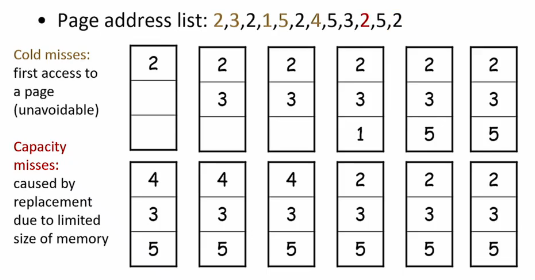
\includegraphics[width=0.75\linewidth]{BeladysAlgorithm} 
  % \caption{An example image}
  % \label{fig:example}
\end{figure}

Timestamp: 11:38

{\bf First-In First-Out (FIFO).} {In this algorithm we would maintain a list of pages in chronological order, and on replacement we would evict the oldest page in the queue.}
    \begin{enumerate}
        \item[]{\bf Pros.} {Maybe the oldest page is not being used. This queue is possible to implement in real life, and it is easy to do so.}
        \item[]{\bf Cons.} {No information about a page except its age in memory. This algorithm also suffers from Belady's Anomaly. The fault rate might actually increase when the algorithm is given more memory.} 
    \end{enumerate}

\begin{figure}[htbp]
  \centering
  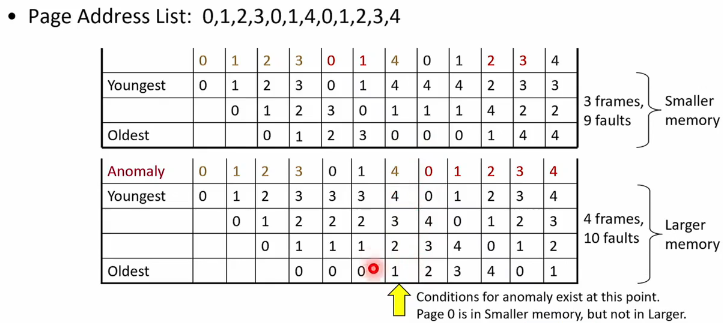
\includegraphics[width=0.75\linewidth]{FIFOReplacement} 
\end{figure}
\vspace{4em}
{\bf Belady's Anomaly.} {It is when the fault rate may increase when an algorithm is given more memory.}
    \begin{enumerate}
        \item[]{\bf The 2 Conditions for a Belady's Anomaly.}
        \begin{enumerate}
            \item[1]{When the larger memory contains at least 1 page that is also in the smaller memory.}
            \item[2]{When the smaller memory contains at least 1 page that is not in the larger memory.} 
        \end{enumerate}
    \end{enumerate}

{\bf Page Fault.} {When a page is not in memory. A page fault can signal a page replacement algorithm.}

{\bf Least Recently Used (LRU)} {The idea is that we can't predict the future, but we can guess based on passed experience. We evict the least recently used page.}
    \begin{enumerate}
        \item[]{\bf Pros.} {Any program with high temporal locality will work well with this algorithm. Eg. code pages or stack pages are used more frequently}
        \item[]{\bf Cons.} {A program with poor temporal locality will not work well with this algorithm. Eg. A program w/ repeated sequential array access larger than avaialable memory. Also this is not easy to implement in reality.}
    \end{enumerate}

{\bf Temporal Locality.} {This refers to the same page/address being accessed frequently.}

{\bf Implementing Exact LRU} {Exact means if we were to implement this on a real computer.}
    \begin{enumerate}
        \item[]{\bf Option 1.} {Have a timestamp so every time we reference the memory, we update the timestamp. We then evict pages with the oldest timestamp, but we'll also have to go through each page in to find one with the oldest timestamp (Problem:O(n)). We'll need to make the page table entry (PTE) large enough to hold a meaningful timestamp. This may double the size of our page tables and TLBs.}
        \item[]{\bf Option 2.} {}
    \end{enumerate}

Timestamp: 25:10


\newpage
\section{Lecture 12: Paging and Address Translation {\hrule}} 

\vspace{-1.5em}

{\bf Compaction.} {The idea that we have something called a physical memory (RAM) and as we are assigning physical memory to processes, we can end up with holes inbetween allocations of memory. The purpose of compaction is to eliminate the small fragments in physical memory by relocating allocated space by consolidating them so we get 1 big free space in physical memory that we can use for other processes.}
    \begin{enumerate}
        \item[]{\bf Note.} {Compaction is not possible with the C memory allocation library. The C library uses something called dynamic partitioning. It's not possible because once malloc() returns an address to you, that address would be out of reach by the malloc library––this means that the malloc library cannot change the address that was returned and update it to something else.}
        \item[] {\bf Dynamic Partitioning.} {Opposite of fixed partitions. \href{run:https://www.youtube.com/watch?v=bQVARMOIwFg}{Video} }
    \end{enumerate}
\vspace{1em}

{\bf Dynamic Relocation.} {Also known as execution-time binding of addresses. The purpose of this is to be able to do {\bf swapping} and {\bf compaction} at runtime. Dynamic relocation allows us to take a virtual address that the user process is using as its executing instructions and translating them to physical addresses.}
    \begin{enumerate}
        \item[]{\bf Note.} {This allows the OS to change the mapping between virtual and physical addresses whenever it wants––thus able to move data from one region of memory to another region of memory.}
        \item[] {\bf Regarding Compaction.} {We are able to change some of the virtual-to-physical address translations.}
        \item[] {\bf What's the minimum requirements to relocate fixed or dynamic partitions?} 
        \vspace{-0.5em}
        \begin{enumerate}
            \item[] All memory used by the process must be contiguous, which means no holes. 
        \end{enumerate}
    \end{enumerate}
\vspace{1em}

{\bf Relocation Registers.} {What some CPU architectures, commonly, the older ones have. The basic idea is to translate physical addresses by doing an add opertation to the virtual address to get the corressponding physical address. }
    \begin{enumerate}
        \item[]{\bf Eg. Translating Addresses w/ Reloc. Reg.} {Let's say base address is 10, and we want to translate the virtual address 5. Then the physical address you get is 10+5 = 15. }
        \item[]{\bf Note.} {We also have to check that the base address is within the limits of a process's address space to protect overwriting memory that we lost to other processes. Sometimes the generated physical address does not even exist, eg. -200 physical address. }
        \item[]{\bf Base and Limit Reg.} {On CPUs that have a "base" and "limit" registers, the MMU uses these registers to store the base address and also a limit. These registers are updated whenever we do a kernel level context switch.}
        \begin{enumerate}
            \item[1]{\bf Base.} {When we restore registers for the next process, we load the {\bf base} register with the starting address of the physical address of that process.}
            \item[2]{\bf Limit.} {Limit register is set to the last logical (virtual) address of that process. Purpose is to cap what range of physical addresses are valid.}
            \item[3]{\bf Load/Store.} {When we execute any memory reference instruction like load and store, the hardware will add the base address to the logical address... tbc} 
        \end{enumerate}
        \item[]{\bf Kernel-Level Context Switch.} {When we switch from one process to another.} 
        \item[]{\bf Logical Address.} {It's the same thing as a virtual address.} 
    \end{enumerate}
Timestamp: 8:22

\newpage
\section{Lecture 15/16: Advanced VM Functionalities {\hrule}} 
\vspace{-1.5em}

{\bf Simplified 2Q Algorithm (S2Q).} {This is an algorithm that combines recency and frequency to combat scanning patterns of an array. This is a type of scan-resistant algorithm to get rid of one-time use pages quickly from our main memory.}
    \begin{enumerate}
        \item[]{\bf What do we do each time a page is accesed?} {Every time we reference a page, if the page is already in queue, we promote the page. If the page is not in queue, we add it to the A1 queue. If we see a page again, we move it to the most recently used position of the AMQueue, so it gets evicted last (lowest priority to get evicted).}
        \begin{enumerate}
            \item[]{\bf A1Queue.} {When we have seen the page for the first time, we put in this queue. Pages in this queue can be evicted, so sometimes we put pages that have already been seen, but are already evicted in this queue.} 
            \item[]{\bf AMQueue.} {This is the main queue. This main queue is an RUQueue where we keep most of the pages that are multi-use. Eg. stack pages or code pages}
        \end{enumerate}
        \item[]{\bf What do we do when we want to evict a page?} The basic idea is that if the size of A1Queue is over a particular threshhold that we set, then we evict the oldest page from A1Queue. If the A1Queue is below the threshold, we kick out the least recently used page from AMQueue. 
        \begin{enumerate}
            \item[]{\bf Note.} {In A3, the threshhold is the size of the memory divided by 10 rounded down.}
        \end{enumerate}
        \item[]{\bf Note.} {This algorithm is not practical for implementation because you're removing or inserting from a queue on every single reference. The reason why clock2Q algorithm is possible/practical is because we just have to update one reference bit on every single memory reference, and this is done by the hardware.}
        \item[]{\bf Note.} {The head for A1Queue is oldest page. The head for AMQueue is most recently used page.}
    \end{enumerate}

Timestamp: 19:47

\newpage
\section{Lecture 11: Memory Management {\hrule}} 
\vspace{-1.5em}

{\bf Memory Management Unit (MMU).} {Memory system must see physical (real) addresses to fetch data or instruction. The MMU is where translation for virtual to physical addresses occur. For every virtual address, physical memory must be allocated. }
    \begin{enumerate}
        \item[]{\bf Note.} {We want to minimize wasted memory. We don't want to allocate physical memory for unused memory in the virtual address space of a process. Eg. Wasted memory is like a hello world program where there's so much space inbetween the heap and stack that's unused :( }
    \end{enumerate}

{\bf Memory Management Goals.}
    \begin{enumerate}
        \item[1] {\bf Virtualization.} {Allow for virtualization of memory, the OS must figure out how to share the main physical real memory.}
        \item[2] {\bf Busy CPU.} {We want to support enough active processes to keep our CPU busy.}
        \item[3] {\bf Memory Efficiency.} {We want to minimize wasted memory.}
        \item[4] {\bf Overhead.} {We want to minimize memory management overhead, which just means to minimize wasted CPU/memory. We want our data structure to track physical memory usage to be as small and as fast as possible.} 
    \end{enumerate}

{\bf The 5 Basic Requirements to Support User Processes}
    \begin{enumerate}
        \item[1]{\bf Relocation.}
        \item[2]{\bf Protection.} 
    \end{enumerate}

Timestamp: 9:18

\newpage
\section{Lecture 9: Scheduling {\hrule}} 
\vspace{-1.5em}

{\bf Process Scheduling.} {The allocation of processors (CPU) to processes/threads overtime.}
    \begin{enumerate}
        \item[] {\bf Note.} {This is the key to multiprogramming: can increase CPU utlization and system throughput by overlapping I/O and computation and make progress on multiple tasks concurrently. (Even on a single-core)}
        \item[] {\bf Throughput.} {The amount of work/items/material passed/done by a system/CPU/process.}
    \end{enumerate}
Timestamp: 5:05 

{\bf Scheduling Building Blocks}
    \begin{enumerate}
        \item[]{\bf Target.} {Kernel-level threads.}
        \item[]{\bf Mechanisms.} {The mechanisms behind sheduling involves the OS trackings various threads by using thread states and thread queues. Eg. Ready queue, block queue, running/execute queue.}  
        \item[]{\bf Policies.} {When we are talking about scheduling, we're talking about the policies of CPU virtualization––which thread to run next and when?} 
        \item[]{\bf Metrics.} {We need metrics to evaluate the effectivness of the scheduler and scheduling algorithms that we choose.}
        \begin{enumerate}
            \item[1] {\bf Performance.} {We look at CPU utlization, where we make sure that the CPU is kept busy when there's work to be done. We also look at throughput, where we want to maximize tasks completed per unit time.} 
            \item[2] {\bf Fairness.} {Ensure that each thread gets a reasonable share of the CPU time, preventing starvation.} 
        \end{enumerate}
    \end{enumerate}

{\bf A Simple Policy.} {Assume that tasks run to completion when they are first scheduled, meaning we never context switch unless they perform a blocking call. Once a thread is done, they make the exit() system call.}
    \begin{enumerate}
        \item[]{\bf Goal.} {Minimize average wait time.}
        \item[]{\bf Arrival Time.} {When a thread becomes ready to run.}
        \item[]{\bf Service Time.} {The amount of time required to run a thread to completion.}
        \item[]{\bf Wait Time.} {The time between a thread's arrival and being scheduled.}
        \item[]{\bf Turnaround Time.} {The time between a threads arrival and completion–– Wait Time + Service Time = Turnaround Time.}  
    \end{enumerate}

{\bf First Come First Served (FCFS)} {Schedules the first thread that's in the wait queue. Uses a first in first out (FIFO) queue.}
\begin{figure}[htbp]
  \centering
  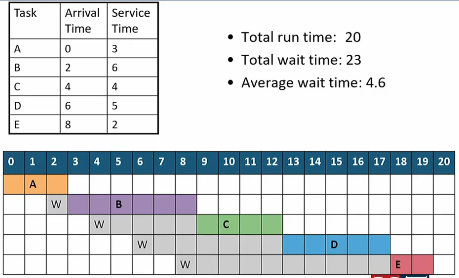
\includegraphics[width=0.75\linewidth]{FCFSScheduling} 
\end{figure}
\vspace{1em}
    \begin{enumerate}
        \item[]{\bf Non-Preemptive.} {Once a task is scheduled in the CPU, it's going to complete with no interruption.}
        \item[]{\bf Con.} {The average wait time w/ FCFS is often quite long due to the convoy effect. Not great if you have a lot of short tasks and 1 big task paired together. If there's a {\bf big variability} in the service time for each task, then this algorithm is pretty bad to use.} 
        \item[]{\bf When to use?.} {When there's not a lot of variability in the service time for each task.} 
    \end{enumerate}

{\bf Shortest Job First {SJF}} {The next thread that is scheduled to run is the thread with the shortest service time.}

{\bf Convoy Effect.} {It's when all other tasks wait for the one "big" task to release the CPU.}

Timestamp: 19:22

\newpage
\section{Lecture 13/14: Translation Lookaside Buffer (TLB) {\hrule}} 
\vspace{-1.5em}

{\bf Segmented Paging.} {The idea that each region of the address space has its own page table.}
    \begin{enumerate}
        \item[]{\bf Eg.} {The code region has its own page table, the stack has its own page table.}
        \item[]{\bf The CONS of segmented paging.}
        \begin{enumerate}
            \item[1]{\bf Page Table Waste.} {Number of valid page table entries can change over time. Eg. sbrk() allows you to adjust the size of the heap, later on we can choose to do a negative sbrk(), shrinking the size of the heap. Eg. We can have a large but sparse heap.} 
            \item[2]{\bf Inflexible.} {The number of regions we can have is limited by the hardware.} 
            \item[3]{\bf Hardware.} {We will need multiple page tables: stackPT, heapPT, dataPT, and code PT. For each region, the hardware will need to use two registers: base and limit. The limit register is used to tell us how big the segment is. Issue: we don't knowhow many regions are in a process. The hardware needed for segmented paging does not exist on any modern CPUs.} 
            \item[4]{\bf External Fragmentation.} {Each page table must be contiguous is some sort of memory (kernel virtual memory or physical memory), but with segmented paging, finding free space for page tables in memory is difficult––difficult to do compaction in the kernel/physical address space.}
        \end{enumerate}
        \item[]{\bf Note.} {We should avoid using contiguous allocations for page tables to avoid dealing with external fragmentation. Therefore segmented paging is a BAD IDEA.}
    \end{enumerate}

{\bf Sparse Heap Page Table.} {A heap page table with a lot of invalid page table entries, resulting in page table waste.}

{\bf Hierarchical Page Table.} {Based on the idea of adding multiple levels of indirection, which is based on the intuition that we don't want to allocate memory for parts of the page table that's not in use.}

Timestamp: 6:33

\newpage
\section{Lecture 14: Paged Virtual Memory {\hrule}} 
\vspace{-1.5em}

{\bf Translation Lookaside Buffer (TLB).} {The input to the TLB is the VPN, and the output is the PFN. This is assuming that the valid bit is set in the PTE and that the operation (R/W) is permitted.}
    \begin{enumerate}
        \item[]{\bf Note.} {The TLB will return an error if we try to write to a page that is set to read only.}
        \item[]{\bf Note 2.} {Because the TLB is very small we have to use it effectively, and so we need to do address translations most of the time––get more hits. Doing translations with a page table is much slower than doing it in the TLB. Eg. w/ a 4-level page table, we need 5 memory accesses, and if each memory access is 100 machine cycles, thats 500 machine cycles compared to 1 machine cycle.} 
    \end{enumerate}

{\bf Address Translation w/ TLB.}
\begin{figure}[htbp]
  \centering
  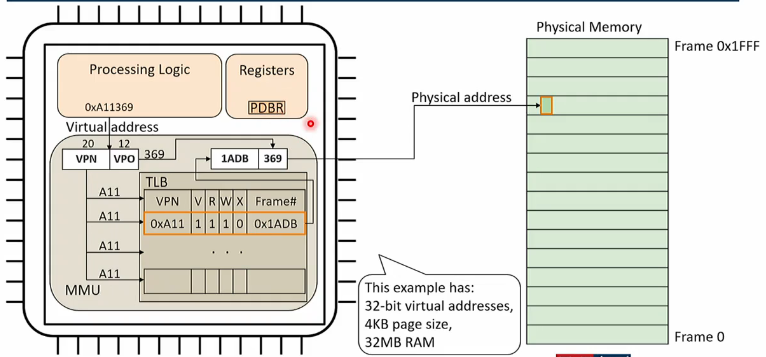
\includegraphics[width=0.75\linewidth]{TLBAddressTranslation} 
  % \caption{An example image}
  % \label{fig:example}
\end{figure}
    \begin{enumerate}
        \item[]{\bf Processing Logic.} {Contains the arithmetic logic unit (ALU) to perform the fetch, decode, execute cycle.}
        \item[]{\bf Registers.} {Contains the page directory base register (PDBR). The PDBR stores a pointer to the page directory that we need to find the page table in memory.} 
        \item[]{\bf MMU.} {Contains the TLB. The TLB will look up the VPN (0xA11 in this example) in all the TLB entries in parallel. The TLB will then use the frame number stored in the 0xA11 VPN TLB entry. In the diagram, since X = 0, if we try to execute an instruction located at the virtual address, a protection fault will occur.}
        \item[]{\bf What happens when we get a TLB miss?} {We use the PDBR to find the page table and then walk the page table to find the page table entry (PTE). After finding the PTE we would update the TLB with a new entry.}  
    \end{enumerate}

{\bf Principle of Locality (Locaility of Reference).} {We get TLB hits most of the time because of this principle. When we look at addresses that are referenced by a process in execution, it turns out only a handful of pages are used at one time, and we only need to have fast translations for the pages that the running process is currently using.}
    \begin{enumerate}
        \item[]{\bf Hits.} {Typically >99\% of translations are hits.}
        \item[]{\bf Misses.} {When we miss a translation it's called a {\bf TLB miss} or {\bf TLB fault}.} 
    \end{enumerate}

{\bf There are 2 ways to handle TLB misses.}
    \begin{enumerate}
        \item[1]{}
        \item[2]{} 
    \end{enumerate}

Timestamp 6:37

\newpage
\section{Lecture 8: Concurrency Bugs {\hrule}} 
\vspace{-1.5em}
{\bf The Three Common Concurrency Bugs.}
    \begin{enumerate}
        \item[1]{\bf Atomicity Violation.} {A bug caused by a lack of mutual exclusion inside the critical section. It happens cause the "desired serializability among multiple memory accesses is violated (eg. a code region should be atomic, but is not). Harder to find cause it does not cause a crash or hang. }
        \begin{enumerate}
            \item[]{\bf Eg.} {Data in your application starts to corrupt slowly.}
        \end{enumerate}
        \item[2]{\bf Order Violation.} {A bug caused by incorrect ordering of operations. Also harder to find because of the same reasons for atomicity violation bugs. Also data starts to corrupt slowly too.}
        \item[3]{\bf Deadlock.} {How to spot: All of the threads would just stop working, when we gdb and take a look, all the threads are sleeping and waiting for some event to happen, but nothing happens.}
        \begin{enumerate}
            \item[]{\bf Eg.} {Your entire website or application just freezes. }
        \end{enumerate}
    \end{enumerate}
\vspace{1em}

{\bf Serializability.} {This is a correctness guarantee that the execution of concurrent operations would be equivalent to some sequential execution of the same operations.}
    \begin{enumerate}
        \item[]{\bf Note.} {Basically the guarantee that mutual exclusion provides.}
        \item[]{\bf Eg.} {$T_A$ executes instructions $a_1, a_2, ..., a_n$ to modify shared data. These instructions are atomic. $T_B$ executes $b_1, b_2, ..., b_n$ to modify the same shared data. The outcome of running $T_A$ and $T_B$ can only be } $a_1, a_2, ..., a_n, b_1, b_2, ..., b_n$ or the otherway around ($T_B$ first then $T_A$).
    \end{enumerate}
\vspace{1em}

{\bf Atomicity Violation: Buggy Code [MySQL]}
    \begin{lstlisting}[language=SQL, numbers=left, basicstyle=\ttfamily]
        Thread 1::
        -- Check if thd.proc_info is null
        if (thd->proc_info) {
            -- If not null, write into thd.proc_info
            fputs(thd->proc_info, ...);
        }
        
        Thread 2::
        -- Set thd.proc_info to null
        thd->proc_info = NULL;
    \end{lstlisting}
    \begin{enumerate}
        \item[1]{\bf What's wrong with this code?} {An interleaving can happen, creating an atomicity violation. Line 3 -> Line 10 -> Crashed Line 5 (cause we can't pass null pointer) is the atomicity violation.}
        \item[2]{\bf How can we fix it?} {Using the same atomic lock() and unlock() on both critical sections.}
    \end{enumerate}

Timestamp: 13:35
\end{document}